\chapter{Programmazione dinamica}

Sappiamo che gli algoritmi basati sulla tecnica del Divide et Impera seguono i 3 punti:
\begin{itemize}
    \item Dividi il problema in sottoproblemi di taglia inferiore.
    \item Risolvi (ricorsivamente) i sottoproblemi di taglia inferiore.
    \item Combina le soluzioni dei sottoproblemi in una soluzione del problema originale. 
\end{itemize}

Negli esempi finora visti i sottoproblemi che si ottenevano dalla applicazione del passo 1 erano tutti diversi, pertanto ciascuno di essi veniva individualmente risolto dalla relativa chiamata ricorsiva del passo 2. In molte situazioni i sottoproblemi ottenuti al passo 1 possono risultare uguali. In tal caso, l'algoritmo basato sulla tecnica del Divide et Impera risolve lo stesso problema più volte svolgendo lavoro inutile.

\begin{redbar}
In termini generali la programmazione dinamica, al pari del divide et impera può essere vista come un metodo che risolve un problema risolvendo problemi di dimensione più piccola e grazie all'utilizzo di tabelle permette di non ricalcolare più volte lo stesso sottoproblema (memoizzazione). I sottoproblemi possono essere risolti a partire dal più grande al più piccolo (approccio top-down) tipico delle versioni ricorsive o dal più piccolo al più grande (approccio bottom-up) tipico delle versioni iterative.
\end{redbar}

La tabella che riporta le soluzioni di tutti i sottoproblemi è stata fin'ora usata solamente per calcolare il valore della soluzione. Può essere usata anche per ritrovare la soluzione. Come vedremo questa è una proprietà generale degli algoritmi di programmazione dinamica: in un primo momento ci si può concentrare sul calcolo del valore della soluzione e successivamente la tabella utilizzata per ottenere questo valore potrà essere usata per ritrovare la soluzione cui quel valore corrisponde. L'idea è di percorrere all'indietro la tabella, a partire dall'elemento che
rappresenta il valore del problema, di elemento in elemento seguendo a ritroso le "decisioni" che hanno portato a determinare quel valore.

\section{Algoritmi di programmazione dinamica}
\subsection{Sequenza dei numeri di Fibonacci}
La sequenza $f_0, f_1, f_2 ...$ dei numeri di Fibonacci è definita dall'equazione di ricorrenza:
\begin{equation*}
    f_i = f_{i-1} + f_{i-2} \textit{ con } f_0 = f_1 = 1        
\end{equation*}
Ad esempio i primi termini della sequenza sono $1, 1, 2, 3, 5, 8, 13,...$.

\textit{Dato un intero $n$ progettare un algoritmo che calcola $f_n$.}

Il primo algoritmo che viene in mente per risolvere il problema è basato sul divide et impera e sfrutta la definizione stessa di numero di Fibonacci.

\begin{lstlisting}[language=Python]
    def fib(n):
        if n<=1:
            return 1
        a=fib(n-1)
        b=fib(n-2)
        return a+b
\end{lstlisting}
La relazione di ricorrenza per il tempo di calcolo dell'algoritmo è:
\begin{equation*}
    T(n)=T(n-1)+T(n-2)+O(1)
\end{equation*}
ovviamente $T(n)\geq 2T(n-2)+O(1)$ e questa ricorrenza può essere facilmente risolta (ad esempio col metodo iterativo) e otteniamo $T(n)=\Omega(2^\frac{n}{2})$.
Il motivo di tale inefficienza sta nel fatto che il programma \verb|fib| viene chiamato sullo stesso input molte volte e ciò è chiaramente ridondante.

\begin{figure}[ht]
    \centering
    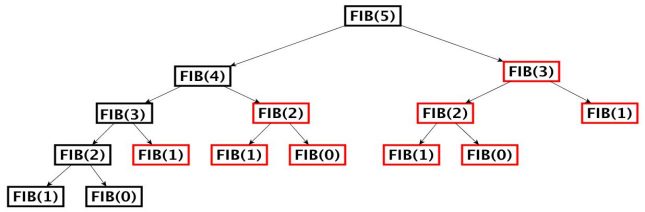
\includegraphics[width=0.7\linewidth]{images/es-fib5.PNG}
    \caption{Chiamate ricorsive per \texttt{fib(5)}}
    \label{fig:es-fib5}
\end{figure}

Nel corso della scomposizione in sottoproblemi, stesse quantità vengono calcolate più volte da differenti chiamate ricorsive. I sottoproblemi in cui viene scomposto il problema non sono disgiunti (questo fenomeno prende il nome di overlapping di sottoproblemi) mentre l'algoritmo si comporta come se lo fossero e li risolve nuovamente.

Individuata la causa dell'inefficienza dell'algoritmo è facile individuare la cura. Basta memorizzare in una lista i valori \verb|fib(i)| quando li si calcola la prima volta cosicché nelle future chiamate ricorsive a \verb|fib(i)| non ci sarà più bisogno di ricalcolarli ma potranno essere ricavati dalla lista (questa tecnica prende il nome di memoizzazione). Si risparmia così tempo di calcolo al costo di un piccolo incremento di occupazione di memoria.

\begin{lstlisting}[language=Python]
    def fib1(n):
        F=[-1]*(n-1)
        return memfib(n, F)

    def memFib(n, F):
        if n<=1:
            return 1
        if F[n]==-1
            a=memFib(n-1, F)
            b=memFib(n-2, F)
            F[n]=a+b
        return F[n]
\end{lstlisting}
La novità dell'algoritmo \verb|fib1| è che esso, prima di attivare la ricorsione per il calcolo di qualche $f_i$, con $i<n$, controlla se quel valore è stato calcolato precedentemente e posto in \verb|F[i]|. In caso affermativo la ricorsione non viene effettuata ma viene restituito direttamente il valore \verb|F[i]|. In questo modo l'algoritmo effettuerà esattamente $n$ chiamate ricorsive (una sola chiamata per il calcolo di ogni $f_i$ con $i<n$). Tenendo conto che ogni chiamata ricorsiva costa $O(1)$ il tempo di calcolo di \verb|fib1| è $\Theta(n)$, un miglioramento esponenziale rispetto alla versione da cui eravamo partiti.

Al punto a cui siamo giunti possiamo anche eliminare la ricorsione ed ottenere la versione iterativa dell'algoritmo.

\begin{lstlisting}[language=Python]
    def Fib2(n):
        F=[-1]*(n+1)
        F[0]=F[1]=1
        for i in range(2, n+1):
            F[i]=F[i-2]+F[i-1]
        return F[n]
\end{lstlisting}
La complessità asintotica rimane $\Theta(n)$ ma abbiamo un risparmio di tempo e spazio (quello necessario alla gestione della ricorsione). La complessità di spazio è $O(n)$ a causa della lista $F$ da memorizzare. Non è difficile ridurre questa occupazione a $\Theta(n)$ tenendo conto che dell'intera tabella basta conservare in memoria volta per volta solo gli ultimi due valori calcolati:

\begin{lstlisting}[language=Python]
    def Fib3(n):
        if n<=1:
            return n
        a=b=1
        for i in range(2, n+1):
            a, b = b, a
        return b
\end{lstlisting}
Riassumendo: siamo partiti da un algoritmo ricorsivo e non efficiente ottenuto applicando la tecnica del divide et impera al problema in esame; ci siamo accorti che il motivo dell'inefficienza era la presenza di overlapping di sottoproblemi; abbiamo risolto il problema del ricalcolo di soluzioni allo stesso sottoproblema mediante la tecnica della memoizzazione e quindi ricorrendo a ”tabelle” per conservare i risultati a sottoproblemi già calcolati; abbiamo sviluppato una versione dell'algoritmo iterativa che ha permesso di sbarazzarsi della ricorsione; abbiamo ottimizzato lo spazio di memoria mantenendo memorizzata nel corso dell'algoritmo solo la parte della tabella che sarebbe servita nel seguito.

Nota che nella versione ricorsiva dell'algoritmo si parte dal problema scomponendolo via via
in sottoproblemi di dimensione sempre più piccola fino ad arrivare a problemi facilmente risolvibili. Si parla in questo caso di approccio top-down al problema. Nella versione iterativa dell'algoritmo si comincia col risolvere i sottoproblemi di dimensione sufficientemente piccola per poi passare a quelli di dimensione via via crescente fino ad arrivare alla soluzione del
problema originario. Si parla in questo caso di approccio bottom-up al problema.

\subsection{Sottoinsieme di file}
\textit{Abbiamo $n$ file di varie dimensioni ciascuna inferiore a $C$ ed un disco di capacità $C$, bisogna trovare il sottoinsieme di file che può essere memorizzato sul disco e che massimizza lo spazio occupato. Progettare un algoritmo che, dati $C$ e lista $A$ dove $A[i]$ è la dimensione del file $i$, risolve il problema.}

Ad esempio, per \verb|C = 100| e \texttt{A = [82, 15, 40, 95, 31, 50, 40, 28]} la risposta deve essere \texttt{{2, 4, 7}} che occupa spazio $40 + 31 + 28 = 99$.

Non è difficile rendersi conto che algoritmi greedy del tipo “finché c'è spazio memorizza sul disco il file di massima dimensione” non trovano sempre la soluzione ottima. Per questo problema non si conoscono algoritmi efficienti. Migliori algoritmi si basano su un qualche tipo di ricerca esaustiva della soluzione. Per fortuna è altrettanto facile trovare algoritmi d'approssimazione efficienti con rapporti d'approssimazione costante.

Per semplicità di esposizione ci limiteremo ora a calcolare il valore della soluzione ottima, cioè il massimo spazio del disco che può essere occupato grazie agli $n$ file. 

Un algoritmo basato sul divide et impera può partire dalla seguenti osservazioni: Sia $(A, C)$ l'istanza che vogliamo risolvere, se la lista dei file risulta vuota o la capacità $C$ vale 0 la soluzione ottima vale 0. In caso contrario l'ultimo file della lista può appartenere o meno alla soluzione ottima. Se l'ultimo file non appartiene alla soluzione i rimanenti $n-1$ file devono essere una soluzione ottima per $(A[:-1], C)$; se l'ultimo file appartiene alla soluzione i rimanenti $n-1$ file devono essere una soluzione ottima per $(A[:-1], C-A[n-1])$.

Possiamo quindi ricondurci al calcolo della soluzione ottima di due sottoproblemi di dimensione inferiore in quanto manca all'appello l'ultimo file e, una volta risolti questi due problemi, ottenuti i valori $v1$ e $v2$ delle loro soluzioni, la soluzione al problema di partenza sarà data da $\max(v1, v2 + A[-1])$.

\begin{minipage}[t]{0.50\textwidth}
\begin{lstlisting}[language=Python]
def es(A, C):
    if len(A)==0 or C==0:
        return 0
    lascio = es(A[:-1], C)
    if A[-1] > C:
        return lascio
    prendo = A[-1] + es(A[:-1], C-A[-1])
    return max(lascio, prendo)
\end{lstlisting}
\end{minipage}
%\hspace{-1cm}
\begin{minipage}[t]{0.50\textwidth}
\begin{lstlisting}[language=Python]
def es(A, i, C):
    if i==0 or C==0:
        return 0
    lascio = es(A, i-1, C)
    if A[i-1] > C:
        return lascio
    prendo = A[i-1] + es(A, i-1, C-A[i-1])
    return max(lascio, prendo)
\end{lstlisting}
\end{minipage}
Con la prima implementazione per la complessità si avrà:
\begin{equation*}
    T(n) = T(n - 1, C) + T(n - 1, C - A[n - 1]) + \Theta(n)
\end{equation*}
il costo addittivo $O(n)$ è dovuto al passaggio della copia della lista.

Con la seconda implementazione per la complessità si avrà:
\begin{equation*}
    T(n) = T(n - 1, C) + T(n - 1, C - A[n - 1]) + \Theta(1)
\end{equation*}
Considera l'istanza in cui $C=n-1$ e $A[i]=1$, $0\leq i\leq n$. Per quest'istanza l'equazione di ricorrenza della seconda implementazione dà:
\begin{align*}
    T(n) = T(n - 1, C) + T(n - 1, C - A[n - 1]) + \Theta(1) \geq 2T(n - 1, n - 1) + \Theta(1) = 2T(n - 1) + \Theta(1)
\end{align*}
che risolta dà $T(n)=\Omega(2^n)$. Il motivo di questi tempi intrattabili è dovuto all'overlapping dei sottoproblemi generati dal partizionamento prodotto dal divide et impera.

Di seguito parte dell'albero di ricorsione generato durante l'esecuzione dell'istanza dove \verb|C = 10| e \texttt{lista = [1, 5, 3, 4, 2, 2]} dove ciascun nodo è una coppia con al primo posto il numero di file dell'istanza ed al secondo la capacità del disco. In rosso sono marcate le chiamate ricorsive duplicate che l'algoritmo ricalcola. Più l'istanza è grande e più chiamate ricorsive duplicate saranno presenti.

\begin{figure}[ht]
    \centering
    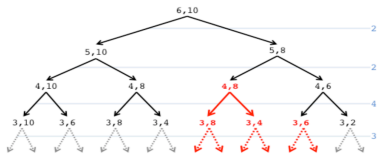
\includegraphics[width=0.6\linewidth]{images/es-file.PNG}
    \caption{Albero di ricorsione del problema}
    \label{fig:es-file}
\end{figure}
Per evitare di fare questo inutile lavoro ricorriamo alla memoizzazione, utilizziamo una tabella in cui salviamo i risultati via via calcolati per poterli riutilizzare se necessario senza doverli ricalcolare. La tabella $T$ avrà dimensione $n\times (C+1)$ e nella cella $T[i][j]$ memorizzeremo il valore ottenuto dalla soluzione del sottoproblema in cui si hanno i soli
primi $i$ file e la dimensione del disco è $j$.

\begin{lstlisting}[language=Python]
    def es(A, C):
        T=[[-1]*(C+1) for i in range(len(A)+1)]
        return mem_es(A, len(A), C, T)
    
    def mem_es(A, i, c, T):
        if T[i][c]==-1:
            if i==0 or C==0:
                T[i][c]=0
            else:
                lascio = mem_es(A, i-1, c, T) 
                T[i][c] = lascio
                if A[i-1] <= c:
                    prendo = A[i-1] + mem_es(A, i-1, c-A[i-1], T)
                    T[i][c] = max(lascio, prendo)                    
        return T[i][c]
\end{lstlisting}
La complessità dell'implementazione memoizzata è dunque $O(nC)$ (in realtà è $\Theta(nC)$ perché la tabella va inizializzata con i valori -1). Il tempo di calcolo della versione memoizzata è limitato dalla dimensione della tabella. Infatti, la funzione \verb|mem_file()| esegue $O(1)$ operazioni in ogni chiamata e il numero totale di chiamate non può superare la dimensione della tabella.

La complessità della versione memoizzata è dunque $\Theta(nC)$, quella dell'algoritmo esaustivo è $O(2^n)$. C'è stato un risparmio? Dipende. Se $C$ è molto grande, ad esempio quando supera $2^n$, la versione memoizzata fa peggio. Però se $C$ non è cosi grande, la versione memoizzata è più efficiente e a volte enormemente più efficiente.

Consideriamo un caso abbastanza realistico: $n = 100.000$ file e capacità $C = 1.000.000$ (assumiamo che le dimensioni dei file e la capacità siano espresse in multipli di MB, cosi $C$ equivale a 1 TB) con dimensione massima dei file 1000 (cioè 1 GB) di modo che qualsiasi sottoinsieme di 1000 file può essere memorizzato sul disco.
L'algoritmo non memorizzato eseguirà tutte le chiamate ricorsive (cioè sarà sempre possibile scegliere il k-esimo file) almeno relativamente ai primi 1000 file (da $n = 100.000$ a $99.000$). Quindi la complessità dell'algoritmo non memorizzato sarà almeno dell'ordine di $2^{1000}$. L'algoritmo memorizzato ha una complessità dell'ordine di $nC = 100.000 * 1.000.000 100.000.000.000$.
Quindi un computer con sufficiente memoria (dell'ordine delle centinaia di GB) potrò eseguire l'algoritmo memorizzato in meno di un'ora. Mentre con l'algoritmo non memorizzato, dovendo eseguire almeno $2^{1000}$ operazioni, anche usando tutti i computer del pianeta, non riusciremo a vedere il risultato del calcolo neanche aspettando fino alla fine all'età stimata dell'universo.

Come mostra l'esempio appena visto la profondità dell'albero delle chiamate ricorsive (in entrambe le versioni dell'algoritmo) può essere molto grande e portare a stack overflow. Nella versione memoizzata ci si può concentrare direttamente sul calcolo della tabella $T$ eliminando così la ricorsione.

Definiamo una tabella $T$ di dimensioni $(n + 1)\times (C + 1)$ dove: $T[i, c]$ = spazio massimo con i primi $i$ file su un disco di capacità $c$ con $0\leq i \leq n$ e $0 \leq c \leq C$. La soluzione al problema originario la troviamo in $T[n][C]$. Possiamo calcolare la tabella per righe grazie alla seguente formula ricorsiva:

\begin{equation*}
    T[i, c]=
    \begin{cases}
        0\hspace{7.8cm}\textit{se }i=0\\
        T[i-1, c]\hspace{6.5cm}\textit{se }c<A[i-1]\\
        max(T[i-1, c], A[i - 1] + T[i-1, c - A[i - 1]])\hspace{.6cm} altrimenti
    \end{cases}
\end{equation*}

\begin{lstlisting}[language=Python]
    def es1(A, C):
        n=len(A)
        T=[[0]*(C+1) for i in range(n+1)]
        for i in range(1, n+1):
            for c in range(C+1):
                if c < A[i-1]:
                    T[i][c] = T[i-1][c]
                else:
                    T[i][c] = max(T[i-1][c], A[i-1]+T[i-1][c-A[i-1]])
        return T[n][C]
\end{lstlisting}
Ha complessità $O(nC)$. In termini dell'albero delle chiamate ricorsive, l'algoritmo iterativo, calcola i risultati a partire dalle foglie, cioè gli elementi $T[0, c]$), poi i risultati del livello superiore e così via risalendo l'albero di livello in livello fino alla radice $T[n, C]$ (approccio bottom-up al problema).
 
L'algoritmo che abbiamo ottenuto di complessità $O(nC)$ è un esempio di algoritmo pseudopolinomiale. Ricorda che la capacità $C$ del disco data in input è codificata con $\log C$ bit e quindi per ottenere un algoritmo polinomiale nella complessità può comparire $\log^c C$ per una qualche costante $c$ la presenza di $C$ nella complessità mostra che questa può essere anche esponenziale nella reale dimensione dell'input.

Consideriamo la tabella $T$ del problema relativamente all’istanza $C = 10$ e 6 file di dimensioni $A = [1, 5, 3, 4, 2, 2]$.

\begin{figure}[ht]
    \centering
    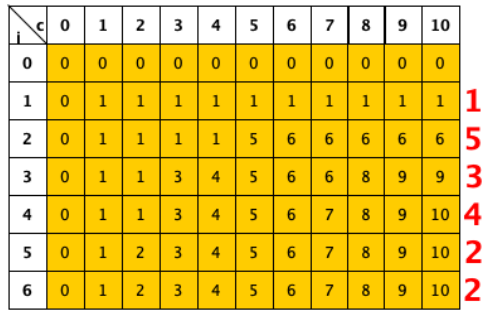
\includegraphics[width=0.5\linewidth]{images/es-tabella-file.PNG}
    \caption{Tabella per il problema dei file}
    \label{fig:es-tabella-file}
\end{figure}

Tenendo conto che la tabella è stata calcolata per mezzo della seguente formula ricorsiva:
\begin{equation*}
    T[i, c]=
    \begin{cases}
        0\hspace{7.8cm}\textit{se }i=0\\
        T[i-1, c]\hspace{6.5cm}\textit{se }c<A[i-1]\\
        max(T[i-1, c], A[i - 1] + T[i-1, c - A[i - 1]])\hspace{.6cm} altrimenti
    \end{cases}
\end{equation*}
Nella tabella a partire da $T[n, C]$ da ogni elemento toccato della tabella $T[k, c]$ è tracciata una freccia verso l’elemento in base al quale è stato calcolato $T[k, c]$ (questo elemento sarà $T[k-1, c]$ o $T[k-1, c-A[k]]$). Quindi se la freccia è verso $T[k-1, c]$ (una freccia verticale) vuol dire che il k-esimo file non è scelto mentre se la freccia è verso $T[k-1, c-A[k]]$ (una freccia obliqua) vuol dire che il k-esimo file è stato scelto.

\begin{figure}[ht]
    \centering
    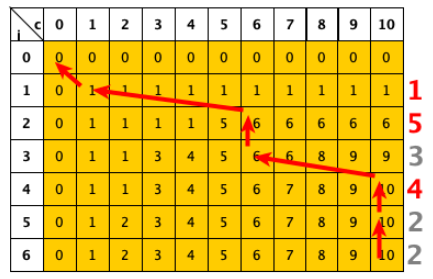
\includegraphics[width=0.5\linewidth]{images/es-tabella-file2.PNG}
    \caption{Tabella per il problema dei file}
    \label{fig:es-tabella-file2}
\end{figure}

Le frecce rosse evidenziano le decisioni a partire dall'elemento $T[n, C]$ che fornisce il valore della soluzione ottima. In base a queste è possibile dire quali file sono stati scelti nella soluzione ottima (i file di dimensioni 4, 5, e 1). Quindi se $T[k, c] = T[k-1, c]$, il k-esimo file non è scelto (nella soluzione del sotto-problema $T[k, c]$), altrimenti $T[k, c] > T[k-1,c]$ e il k-esimo file è stato scelto.

\begin{lstlisting}[language=Python]
    def es1(A, C):
        n=len(A)
        T=[[0]*(C+1) for i in range(n+1)]
        for i in range(1, n+1):
            for c in range(C+1):
                if c < A[i-1]:
                    T[i][c]=T[i-1][c]
                else:
                    T[i][c] = max(T[i-1][c], A[i-1] + T[i-1][c-A[i-1]])

        valore=T[n][C]
        sol=set()
        i=n
        while i > 0:
            if T[i][valore] != T[i-1][valore]:
                sol.add(i-1)
                valore-=A[i-1]
            i-=1
        return T[n][C], sol
\end{lstlisting}
Nella prima parte viene pagato $O(nC)$ per il calcolo della tabella. Nella seconda parte, alla ricerca dei file presenti nella soluzione ottima, la tabella viene visitata a partire dall'ultima cella $T[n, C]$, un riga in meno per volta. Il costo di questa visita è $O(n)$. La complessità è $O(nC)$.

\subsection{Sequenza di zeri in stringhe binarie}
\textit{Dato un intero $n$ vogliamo contare le stringhe binarie lunghe $n$ in cui non compaiono zeri consecutivi. L'algoritmo proposto deve avere complessità $O(n)$.}

Ad esempio per $n=1$ sono 2: $(0, 1)$; per $n=4$ sono 5: $(010, 011, 101, 110, 111)$.

Utilizzeremo una tabella monodimensionale di dimensioni $n+1$ e definiamo il contenuto delle celle come segue: $T[i] =$ numero di stringhe binarie lunghe $i$ dove non compaiono 2 zeri consecutivi. Una volta riempita la tabella la soluzione al nostro problema la troveremo nella locazione $T[n]$. Resta da definire la regola ricorsiva con cui calcolare i valori $T[i]$ nella tabella.
\begin{equation*}T[i]=
    \begin{cases}
        1\hspace{3.6cm}\textit{se } i=0\\
        2\hspace{3.6cm}\textit{se } i=1\\
        T[i-1]+T[i-2]\hspace{1cm}\textit{altrimenti}\\
    \end{cases}
\end{equation*}
La ricorrenza viene fuori dal seguente ragionamento: il conteggio può essere visto come la somma delle stringhe da contare lunghe $i$ che terminano con 1 e le stringhe da contare lunghe $i$ che terminano con 0. Le stringhe da contare lunghe $i$ che terminano con 1 si ottengono accodando la cifra 1 a quelle da contare lunghe $i-1$. Queste stringhe sono $T[i - 1]$. Le stringhe da contare lunghe $i$ che terminano con 0 devono avere al penultimo posto la cifra 1, si ottengono dunque accodando 10 alle stringhe da contare lunghe $i-2$. Queste stringhe sono dunque $T[i-2]$.
\begin{lstlisting}[language=Python]
    def es(n):
        T=[0]*(n+1)
        T[0], T[1] = 1, 2
        for i in range(2, n+1):
            T[i] = T[i-1]+T[i-2]
        return T[n]
\end{lstlisting}

\subsection{Persone in un albergo}
\textit{Dato un intero $n$ vogliamo contare quanti modi diversi ci sono di sistemare $n$ persone in un albergo che dispone di camere singole e camere doppie. L’algoritmo proposto deve avere complessità $\Theta(n)$.}

Ad esempio per $n=2$ sono 2: $\{[1], [2]\} \{[1,2]\}$; per $n=4$ sono 10: $\{[1], [2], [3], [4]\}$ $\{[1,2], [3], [4]\}$ $\{[1,3], [2], [4]\}$ $\{[1,4], [2], [3]\}$ $\{[2,3], [1], [4]\}$ $\{[2,4], [1], [3]\}$ $\{[3,4], [1], [2]\}$ $\{[1,2], [3,4]\}$ $\{[1,3], [2,4]\}$ $\{[1,4], [2,3]\}$.

Utilizzeremo una tabella monodimensionale di dimensioni $n+1$ e definiamo il contenuto delle celle come segue: $T[i] =$ numero di modi in cui è possibile sistemare $i$ persone nell’albergo. Una volta riempita la tabella la soluzione al nostro problema la troveremo nella locazione $T[n]$. Resta da definire la regola ricorsiva con cui calcolare il valore $T[i]$ calcolati i valori $T[j]$ che precedono nella tabella.
\begin{equation*}T[i]=
    \begin{cases}
        1\hspace{5cm}\textit{se } i=0\\
        1\hspace{5cm}\textit{se } i=1\\
        T[i-1]+(i-1)*T[i-2]\hspace{1cm}\textit{altrimenti}\\
    \end{cases}
\end{equation*}
La ricorrenza viene fuori dal seguente ragionamento: possiamo vedere le disposizioni delle $i$ persone come la somma di due diverse tipologie: quelle in cui la persona $i$ finisce in camera da sola e quelle in cui la persona $i$ finisce in camera con una delle altre $i-1$ persone. Le differenti disposizioni in cui $i$ finisce da solo sono $T[i - 1]$, sono infatti tutti i possibili modi di disporre le altre $i - 1$ persone. Le differenti disposizioni in cui $i$ finisce in camera con una delle altre $i-1$ persone sono $(i-1)*T[i-2]$ infatti ci sono $i-1$ modi di scegliere il compagno di stanza e una volta scelto il compagno ci sono $T[i - 2]$ modi di disporre tutte le altre $i - 2$ persone nelle varie camere.
\begin{lstlisting}[language=Python]
    def es3(n):
        T=[0 for _ in range(n+1)]
        T[0]=T[1]=1 
        for i in range(2, n+1):
            T[i] = T[i-1]+(i-1)*T[i-2]
        return T[n]
\end{lstlisting}

\subsection{Somma massima per una sottosequenza}
\textit{Dato un array $A$ di $n\geq 2$ interi positivi vogliamo calcolare la somma massima per una sottosequenza di elementi di $A$ non consecutivi. L'algoritmo proposto deve avere complessità $O(n)$.}

Ad esempio per $A = [5, 4, 2, 10, 6, 8]$ la risposta è 23 infatti per $A$ la sottosequenza di interi non consecutivi di valore massimo è quella di seguito evidenziata in rosso \textcolor{red}{5}, 4, 2, \textcolor{red}{10}, 6, \textcolor{red}{8}.

Utilizzeremo una tabella monodimensionale di dimensioni $n-1$ e definiamo il contenuto delle celle come segue:  $T[i] =$ la somma massima per una sottosequenza di elementi non consecutivi in $A[:i+1]$.
Una volta riempita la tabella la soluzione al problema sarà data da $T[n-1]$. Resta da definire la regola ricorsiva con cui calcolare i valori $T[i]$ della tabella.
\begin{equation*}T[i]=
    \begin{cases}
        A[0]\hspace{4.8cm}\textit{se } i=0\\
        \max(A[0], A[1])\hspace{3cm}\textit{se } i=1\\
        \max(T[i-1], T[i-2] + A[i])\hspace{1cm}\textit{altrimenti}
    \end{cases}
\end{equation*}
La ricorrenza viene fuori dal seguente ragionamento:
\begin{enumerate}
    \item Il vettore contiene un solo elemento allora meglio prenderlo perché positivo $T[0]=A[0]$.
    \item Il vettore contiene due soli elementi allora meglio prendere il più grande dei due $T[1] = \max(A[0], A[1])$.
    \item Alla soluzione di $A[:i+1]$ appartiene l’ultimo elemento $A[i]$. In questo caso l’elemento $A[i-1]$ non può appartenere alla soluzione e quindi il massimo deve essere $T[i - 2] + A[i]$. Se al contrario $A[i]$ non appartiene alla soluzione allora per la soluzione deve aversi $T[i] = T[i - 1]$.

    In generale possiamo quindi dire che $T[i] = \max(T[i - 2] + A[i], T[i - 1])$.
\end{enumerate}
\begin{lstlisting}[language=Python]
    def es(A):
        n=len(A)
        T[0]=A[0]
        T[1] = max(A[0], A[1])
        for i in range(2, n):
            T[i] = max(T[i-1], T[i-2] + A[i])
        return T[n-1]
\end{lstlisting}
Nota che per calcolare un nuovo valore della tabella bastano i due valori precedenti quindi il programma si può migliorare passando dalla complessità di spazio $\Theta(n)$ alla complessità di spazio $\Theta(1)$.

\subsection{Tassellamenti di una superficie}
\textit{Dato l’intero $n$ vogliamo contare il numero di differenti tassellamenti di una superficie di dimensione $n\times 2$ tramite tessere di domino di dimensione $1\times 2$. L'algoritmo deve avere commplessità $O(n)$.}

Ad esempio per $n=1$ la risposta dell'algoritmo deve ovviamente essere 1. Per $n=2$ la risposta deve essere 2 perché sono possibili i soli due seguenti tassellamenti:
\begin{center}
    \begin{tabular}{|c c|}
         \hline x & x\\\hline 
         x & x\\\hline
    \end{tabular}\hspace{1cm}
    \begin{tabular}{|c|c|}
         \hline x & x\\
         x & x\\\hline
    \end{tabular}
\end{center}

Utilizzeremo una tabella monodimensionale di dimensioni $n+1$ e definiamo il contenuto delle celle come segue: $T[i] =$ numero di tassellamenti possibili per la superficie di dimensione $i\times 2$.
Una volta riempita la tabella la soluzione al nostro problema la troveremo nella locazione $T[n]$.
Resta da definire la regola ricorsiva con cui calcolare i valori $T[i]$ nella tabella.
\begin{equation*}T[i]=
    \begin{cases}
        1\hspace{3.6cm}\textit{se } i=0\\
        2\hspace{3.6cm}\textit{se } i=1\\
        T[i-1]+T[i-2]\hspace{1cm}\textit{altrimenti}\\
    \end{cases}
\end{equation*}
La ricorrenza viene fuori dal seguente ragionamento: possiamo vedere i tassellamenti della superficie di dimensione $i\times 2$ come la somma di due diverse tipologie. I tassellamenti in cui il tassello che copre l’ultima cella in basso a sinistra è posizionato in orizzontale e i
tassellamenti in cui il tassello che copre l’ultima cella in basso a sinistra è posizionato in verticale. I tassellamenti in cui il tassello che copre l’ultima cella in basso a sinistra è posizionato in orizzontale sono $T[i - 1]$, infatti il tassello occupa l’i-esima riga della superficie e resta da tassellare una superficie di dimensione $(i - 1)\times 2$ (le prime $i - 1$ righe della superficie) in tutti i modi possibili. Questi modi sono appunto $T[i - 1]$. I tassellamenti in cui il tassello che copre l’ultima cella in basso a sinistra è posizionato in verticale sono $T[i - 2]$ infatti in questo caso il vertice in basso a destra deve essere anch’esso coperto da un tassello in verticale, questi due tasselli lasciano da coprire una superficie di dimensione $(i - 2)\times 2$ (la prime $i - 2$ righe della superficie iniziale) in tutti i modi possibili. Questi modi sono appunto $T[i - 1]$.

\begin{lstlisting}[language=Python]
    def es(n):
        m = max(3, n)
        T = [0]*(n+1)
        T[1], T[2] = 1, 2
        for i in range(3, n+1):
            T[i] = T[i-1] + T[i-2]
        return T[n]
\end{lstlisting}

\subsection{Massimo vettore}
\textit{Data una lista A di $n$ interi, vogliamo trovare una sottolista (una sequenza di elementi consecutivi della lista) la somma dei cui elementi è massima.}

\begin{figure}[ht]
    \centering
    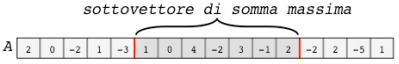
\includegraphics[width=0.5\linewidth]{images/es-sottolista.PNG}
    \caption{Sottolista che contiene valori positivi e negativi}
    \label{fig:es-sottolista}
\end{figure}

Abbiamo già parlato di questo problema come esempio di applicazione della tecnica del divide et impera, lo riprendiamo ora per tentare un approccio basato sulla programmazione dinamica. Come è tipico di questa tecnica ci concentriamo prima sul calcolare il valore della soluzione.

Cominciamo con l’individuare i sottoproblemi dalla composizione delle cui soluzioni sarà poi possibile risolvere il problema originario. Una scelta che ci porta a definire $n$ sottoproblemi è la seguente: $T[i] =$ massima somma possibile per le sottoliste di A che terminano nella posizione $i$. Poichè la sottolista a valore massimo deve terminare in una qualche posizione il valore della soluzione che cerchiamo sarà poi dato da $\max_{0\leq i< n}T[i]$.

Vediamo ora come risolvere in modo efficiente gli $n$ sottoproblemi. Il caso base è facile: $T[0] = A[0]$. Dobbiamo ora poter calcolare $T[i]$, con $i > 0$, sfruttando la conoscenza di $T[i - 1]$:
\begin{equation*}
    T[i] = \max(A[i], A[i] + T[i - 1])
\end{equation*}
Infatti la sottolista di valore massimo che termina con $A[i]$ può essere di due soli tipi: consiste del solo elemento $A[i]$ o ha lunghezza superiore ad 1. In questo caso vale $A[i] + S$ dove $S$ è la massima somma di un sottovettore che termina in $i - 1$ (il che significa che $S = T[i - 1]$).

\begin{lstlisting}[language=Python]
    def es(A):
        T = [0]*n
        for i in range(1, n):
            T[i] = max(A[i], A[i]+T[i-1])
        return max(T)
\end{lstlisting}
Possiamo evitare di dover calcolare al termine il massimo in T, basta una variabile $m$ che tiene traccia del massimo per il valore delle celle di T che via via calcoliamo. Possiamo evitare di tenere in memoria l’intera tabella T visto che per calcolare $T[i]$ basta disporre della sola cella $T[i - 1]$ (e del valore $A[i]$) (in questo modo la complessità di spazio passa da $O(n)$ ad $O(1)$).

\begin{lstlisting}[language=Python]
    def es(A):
        n=len(A)
        m=t= 0
        for i in range(1, n):
            t = max(A[i], A[i]+t)
            m = max(m, t)
        return m
\end{lstlisting}

\subsection{Sottosequenza crescente più lunga}
Data una sequenza di $S$ elementi una sottosequenza di $S$ si ottiene eliminando zero o più elementi da $S$ (non necessariamente le eliminazioni devono avvenire in testa o in coda alla sequenza). Ad esempio: data la sequenza $9, 3, 2, 4, 1, 5, 8, 6, 7, 2$ una sua sottosequenza è $3, 1, 5, 6$ (si ottiene eliminando dalla sequenza gli elementi di seguito indicati in rosso $\textcolor{red}{9},3,\textcolor{red}{2},\textcolor{red}{4},1,5,\textcolor{red}{8},6,\textcolor{red}{7},\textcolor{red}{2}$). Le sottosequenze possibili per una sequenza di elementi sono $\Theta(2^n)$. Una sottosequenza è detta crescente se i suoi elementi risultano ordinati in modo crescente.

\textit{Data una sequenza $S$ di $n$ interi, vogliamo trovare la lunghezza massima per le sottosequenze crescenti presenti in $S$. Progettare un algoritmo che data una sequenza $S$ di $n$ elementi, in tempo $O(n^2)$ risolve il problema.}

Ad esempio: per la sequenza $S = 9, 3, 2, 4, 1, 5, 8, 6, 7, 2$ la risposta è 5 infatti la sottosequenza più lunga in $S$ è $3, 4, 5, 6, 7$ (non è l'unica, un'altra possibile soluzione è $2, 4, 5, 6, 7$).

Utilizzeremo una tabella monodimensionale di dimensioni $n$ e definiamo il contenuto delle celle come segue: $T[i] =$ la lunghezza massima per una sottosequenza crescente che termina con l’elemento di $S$ in posizione $i$. Poiché la sottosequenza di lunghezza massima da qualche parte dovrà pur terminare la soluzione al nostro problema sarà data da: $\max_{0\leq i<n}(T[i])$. Resta da definire la regola ricorsiva con cui calcolare i valori $T[i]$ nella tabella.
\begin{equation*}T[i]=
    \begin{cases}
        1\hspace{5cm}\textit{se }S_j>S_i\textit{ per }0\leq j<i\\
        \max_{0\leq j<i\textit{ con }S_j<S_i}(T[j])+1\hspace{1cm}\textit{altrimenti}
    \end{cases}
\end{equation*}
La ricorrenza viene fuori dal seguente ragionamento: se tutti gli elementi che precedono $S_i$ sono maggiori di $S_i$ allora l’unica sottosequenza crescente che termina in posizione $i$ è data dal solo elemento $S_i$; in caso contrario la sottosequenza che termina con $S_i$ avrà come prefisso una sottosequenza crescente che termina in una posizione $j$ con $j<i$ e $S_j \leq S_i$ e tra tutti i possibili ”agganci” prendo quello che produce la sottosequenza più lunga.

\begin{lstlisting}[language=Python]
    def es(A):
        n=len(A)
        if n==0:
            return 0
        T=[1]*n
        for i in range(1, n):
            for j in range(i):
                if A[i] > A[j]:
                    T[i] = max(T[i], T[j]+1)
        return max(T)
\end{lstlisting}

\subsection{Quadrati di un numero}
Un numero intero può sempre essere rappresentato come somma di quadrati di altri numeri interi. Infatti, usando il quadrato $1^n$, il generico numero $x$ possiamo sempre scomporlo come somma di $n$ addendi tutti uguali a $1^2$ (vale a dire $x = 1^2 + ... + 1^2$).

\textit{Dato un intero $n$ vogliamo sapere qual'è il numero minimo di quadrati necessari rappresentare $n$. Progettare un algoritmo che dato $n$ in $\Theta(n^{\frac{3}{2}})$ calcola il numero minimo di quadrati che servono per rappresentarlo.}

Ad esempio per $n=0$ la risposta è 0. Per $n=41$ la risposta è 2 infatti $41=5^2+4^2$. Nota che vale anche $41=6^2+2^2+1^2$ ma questa scomposizione usa 3 quadrati e non è minimale. Per $n=6$ la risposta è 3 infatti $6=2^2+1^2+1^2$ e non è difficile vedere che 6 non può esprimersi come somma di due soli quadrati.

Utilizzeremo una tabella monodimensionale di dimensioni $n+1$ e definiamo il contenuto delle celle come segue: $T[i] =$ numero minimo di quadrati per rappresentare l’intero $i$. Una volta riempita la tabella troveremo la soluzione in $T[n]$. Resta da definire la regola ricorsiva con cui calcolare i valori $T[i]$ nella tabella.
\begin{equation*}T[i]=
    \begin{cases}
        0\hspace{4.7cm}\textit{se }i=0\\
        \max_{0\leq j\leq \sqrt{i}}(T[i-j^2])+1\hspace{1cm}\textit{altrimenti}
    \end{cases}
\end{equation*}
La ricorrenza viene fuori dal seguente ragionamento: per $i = 0$ ovviamente vale $T[0] = 0$. Per il caso generale dove $i > 0$ servirà utilizzare almeno un quadrato. Tra tutti i quadrati potenzialmente utili ad ottenere $i$ servirà dunque trovare quello che poi permette di ottenere $i$ con il minor numero di quadrati. I quadrati potenzialmente utili sono del tipo $j$ con $1\leq j \leq \sqrt{i}$ e, notando che se si usa il quadrato $j$ resterà poi ancora da rappresentare il numero $i - j^2$ si ottiene la seguente formula: $T[i] = \min_{i\leq j\leq \sqrt{i}}T[i - j^2] + 1$.

\begin{lstlisting}[language=Python]
    def es(n):
        T=[0]*(n+1)
        for i in range(1, n+1):
            T[i]=n
            j=1
            while j**2 <= i:
                if T[i-j**2]+1 < T[i]:
                    T[i] = T[i-j**2]+1
                j+=1
        return T[n]
\end{lstlisting}

\subsection{Sequenze decimali non decrescenti}
\textit{Dato un intero $n$ vogliamo sapere quante sono le sequenze di cifre decimali non decrescenti lunghe $n$. Progettare un algoritmo che trova la risposta in tempo $O(n)$.}

Ad esempio per $n=1$ la risposta dell'algoritmo deve ovviamente essere 10, per $n=2$ la risposta deve essere 55. Infatti alla cifra $x$ al primo posto possono seguire $10-x$ cifre diverse. Quindi si ha
\begin{equation*}
    \sum^9_{x=0}(10-x)=\sum^{10}_{i=1}i=\frac{10*11}{2}=55
\end{equation*}
Utilizzeremo una tabella bidimensionale di dimensioni $n\times 10$ e definiamo il contenuto delle celle come segue: $T[i][j] =$ numero di sequenze decimali non decrescenti lunghe $i$ che terminano con la cifra $j$. Una volta riempita la tabella la soluzione al nostro problema sarà data dalla somma degli elementi nell'ultima riga: $\sum^9_{j=0}T[n][j]$.
Resta da definire la regola ricorsiva con cui calcolare i valori $T[i][j]$ della tabella:
\begin{equation*}T[i][j]=
    \begin{cases}
        1\hspace{3.2cm}\textit{se }i=1\\
        \sum^j_{i=0}T[i-1][k]\hspace{1cm}\textit{altrimenti}
    \end{cases}
\end{equation*}
La ricorrenza viene fuori dal seguente ragionamento: esiste un'unica sequenza lunga 1 che termina con la cifra $j$, la cifra $j$ ed è ovviamente non decrescente. La sequenza lunga $i$ non decrescente che termina con $j$ è composta da una sequenza non decrescente lunga $i-1$ cui si accoda la cifra $j$. Perché la sequenza risultante sia non decrescente la sequenza non decrescente lunga $i-1$ deve terminare con una qualunque cifra $k$ non superiore a $j$ (vale a dire: deve essere una della sequenza contata con $T[i-1, k]$ e $k\leq j$).

\begin{lstlisting}[language=Python]
    def es(n):
        T = [[0]*10 for _ in range(n+1)]
        for j in range(10):
            T[1][j]=1
        for i in range(2, n+1):
            for j in range(10):
                for k in range(j+1):
                    T[i][j] += T[i-1][k]
        return sum(T[n])
\end{lstlisting}
Inizializzare la tabella costa $\Theta(n)$ (nota che la tabella ha $n+1$ righe ma un numero costante di colonne: 10). Dei 3 for annidati il primo viene iterato esattamente $n$ volte, il secondo viene ogni volta iterato esattamente 10 volte ed il terzo viene iterato ogni volta al più 10 volte. Questo significa che il costo totale dei 3 for è $\Theta(n)$.

\subsection{Percorso nella matrice}
\textit{Data una matrice $M$ binaria $n\times n$ vogliamo verificare se nella matrice è possibile raggiungere la cella in basso a destra partendo da quella in alto a sinistra senza mai toccare celle che contengono il numero 1. Si può assumere che $M[0][0] = 0$. Si tenga conto che ad ogni passo ci si può spostare solo di un passo verso destra o un passo verso il basso. Progettare un algoritmo che in tempo $\Theta(n^2)$ risolve il problema rispondendo True o False.}

Ad esempio per la matrice A la risposta è si mentre per la matrice B la risposta è no.
\begin{center}$A=$
    \begin{tabular}{|c|c|c|c|c|c|}
         \hline \textcolor{red}{0}&\textcolor{red}{0}&\textcolor{red}{0}&0&0&1\\\hline
         0&1&\textcolor{red}{0}&1&1&1\\\hline
         0&0&\textcolor{red}{0}&1&0&1\\\hline
         0&1&\textcolor{red}{0}&\textcolor{red}{0}&\textcolor{red}{0}&\textcolor{red}{0}\\\hline
         0&0&0&0&1&\textcolor{red}{0}\\\hline
         1&1&0&1&0&\textcolor{red}{0}\\\hline
    \end{tabular}\hspace{1cm}
    $B=$
    \begin{tabular}{|c|c|c|c|c|c|}
         \hline 0&0&0&0&0&0\\\hline
         0&1&1&1&0&0\\\hline
         0&1&0&0&0&0\\\hline
         0&1&0&1&1&1\\\hline
         0&1&0&0&0&0\\\hline
         0&0&0&0&1&0\\\hline
    \end{tabular}
\end{center}
Utilizziamo una tabella $T$ bidimensionale $n\times n$ dove $T[i][j] = True$ se esiste un cammino che in $M$ va dalla cella $M[0][0]$ in alto a sinistra e arriva alla cella $M[i][j]$ senza toccare celle con valore 1 ($False$ altrimenti). La soluzione al problema sarà nella cella $T[n - 1][n - 1]$.

Ecco di seguito la regola ricorsiva che permette di calcolare i valori della tabella
\begin{equation*}
    T[i][j]=
    \begin{cases}
        False\hspace{3.7cm}\textit{se }M[i][j]=1\\
        True\hspace{3.8cm}\textit{se }i=j=0\\
        T[i][j-1]\hspace{3cm}\textit{se }i=0\\
        T[i-1][j]\hspace{3cm}\textit{se }j=0\\
        T[i][j-1] \textit{ or } T[i-1][j]\hspace{1cm}\textit{altrimenti}
    \end{cases}
\end{equation*}
La ricorrenza viene fuori dal seguente ragionamento: la cella $M[0][0]$ è ovviamente raggiungibile; se la cella $M[i][j]$ contiene 1 allora non è possibile raggiungerla. Assumiamo quindi nel seguito che $M[i][j]=0$. Una cella della prima riga può essere raggiunta solo dalla cella che la precede sulla riga. Una cella della prima colonna può essere raggiunta solo dalla cella che la precede sulla colonna. Una cella "interna" è raggiungibile se posso raggiungerla dalla cella che la precede sulla riga e/o dalla cella che la precede sulla colonna.

\begin{lstlisting}[language=Python]
    def es (M):
        n=len(M)
        T = [[True]*n for _ in range(n)]
        for j in range(1,n):
            T[0][j] = T[0][j-1]
            if M[0][j]==1:
                T[0][j] = False
        for i in range(1,n):
            T[i][0] = T[i-1][0]
            if M[i][0]==1:
                T[i][0] = False
        for i in range(1,n):
            for j in range(1,n):
                T[i][j] = T[i-1][j] or T[i][j-1]
                if M[i][j]==1:
                    T[i][j] = False
        return T[n-1][n-1]
\end{lstlisting}

\subsection{Sottomatrici quadrate di dimensione massima}
\textit{Abbiamo una matrice quadrata binaria $M$ di dimensione $n\times n$ e vogliamo sapere qual è la dimensione massima per le sottomatrici quadrate di soli uni contenute in $M$. Progettare un algoritmo che data la matrice $M$ restituisce il massimo intero $l$ per cui la matrice $l\times l$ è una sottomatrice di soli uni di $M$. L'algoritmo deve avere complessità $O(n^2)$.}

Ad esempio, per la matrice $M$ in figura la risposta è 3:
\begin{center}$M=$
\begin{tabular}{|c|c|c|c|c|}
     \hline 1&0&1&1&1\\\hline
     \textcolor{red}{1}&\textcolor{red}{1}&\textcolor{red}{1}&1&1\\\hline
     \textcolor{red}{1}&\textcolor{red}{1}&\textcolor{red}{1}&0&1\\\hline
     \textcolor{red}{1}&\textcolor{red}{1}&\textcolor{red}{1}&1&1\\\hline
     1&1&0&1&1\\\hline
\end{tabular}
\end{center}
Utilizziamo una tabella $T$ bidimensionale $n\times n$ dove: $T[i][j] =$ il lato della matrice quadrata più grande contenente tutti uni e con cella in basso a destra $M[i][j]$ (se $M[i][j]=0$ allora $T[i][j]=0$). La soluzione al nostro problema sarà il massimo tra i valori della tabella. Ecco di seguito la regola ricorsiva che permette di calcolare i vari valori della tabella:
\begin{equation*}T[i][j]=
\begin{cases}
    0\hspace{7.7cm}\textit{se }M[i][j]=0\\
    \min\{T[i][j - 1], T[i - 1][j - 1], T[i - 1][j]\}+1\hspace{.8cm}\textit{altrimenti}
\end{cases}
\end{equation*}
La ricorrenza viene fuori dal seguente ragionamento: se $M[i][j] = 0$ allora il rettangolo di tutti uni che ha come cella in basso a destra quella cella ha lato zero. Se $M[i][j] = 1$ allora il lato del rettangolo di soli uni che ha come cella in basso a destra quella cella non può superare $T[i-1][j] + 1$ né $T[i][j - 1] + 1$ né $T[i - 1][j - 1] + 1$ ne segue che il lato di quel rettangolo è al più $\min\{T[i][j - 1], T[i - 1][j - 1], T[i - 1][j]\} + 1$ d'altra parte non è difficile vedere che preso $l=\min\{T[i][j - 1], T[i - 1][j - 1] ,T[i-1][j]\}$ allora il rettangolo di lato $l+1$ con cella in basso a destra $M[i][j]$ è un rettangolo contenente solo uni.
\begin{lstlisting}[language=Python]
    def es(M):
        n=len(M)
        T = [[0]*n for _ in range(n)]
        for i in range(n):
            for j in range(n):
                if M[i][j]==0:
                    T[i][j]=0
                else:
                    T[i][j] = min(T[i][j-1], T[i-1][j-1], T[i-1][j])+1
        m=0
        for i in range(n):
            m = max(m, max(T[i]))
        return m
\end{lstlisting}

\subsection{Problema dello zaino}
\textit{Abbiamo uno zaino di capacità $c$ ed $n$ oggetti, ognuno con un peso $p_i$, e un valore $v_i$. Vogliamo sapere il valore massimo che si può inserire nello zaino. Progettare un algoritmo che, data la capacità $c$ dello zaino e i vettori $P$ (dei pesi) e $V$ (dei valori) degli oggetti, risolve il problema in tempo $O(nc)$.}

Ad esempio, si consideri l'istanza con $c=11$ e $n=5$ oggetti con peso e valore riportati nella seguente tabella:
\begin{center}
\begin{tabular}{|c|c|c|}
     \hline \textbf{oggetto} & \textbf{valore} & \textbf{peso}\\\hline
     1&1&1\\\hline
     2&6&4\\\hline
     3&18&5\\\hline
     4&22&5\\\hline
     5&28&7\\\hline
\end{tabular}
\end{center}
Il sottoinsieme di oggetti $(3,5)$ non è una soluzione ammissibile (perché di peso $12 > C$). Il sottoinsieme di oggetti $(1, 2, 4)$ è una soluzione ammissibile (di peso 10 e valore 29) ma non ottima (perché ne esistono di valore maggiore). Il sottoinsieme di oggetti $(1, 3, 4)$ è una soluzione ammissibile (di peso 11 e valore 41) si può dimostrare che è anche una soluzione ottima.

Utilizziamo una tabella bidimensionale $T$ di dimensione $(n + 1)\times (C + 1)$ dove: $T[i][j] =$ massimo valore ottenibile dai primi $i$ oggetti per uno zaino di capacità $j$. La soluzione al nostro problema sarà $T[n][c]$. Ecco di seguito la regola ricorsiva che permette di calcolare i vari valori della tabella:
\begin{equation*}
\begin{cases}
    0\hspace{6.5cm}\textit{se }i=0\textit{ o }j=0\\
    T[i-1][j]\hspace{5.2cm}\textit{se }p_i>j\\
    \max\{T[i-1][j], v_i+T[i-1][j-p_i]\}\hspace{1cm}\textit{altrimenti}
\end{cases}
\end{equation*}
La ricorrenza viene fuori dal seguente ragionamento: se non si hanno oggetti (vale a dire $i = 0$) o la capacità dello zaino è nulla allora il valore della soluzione sarà 0. Se l'$i$-esimo oggetto ha un peso superiore alla capacità dello zaino (vale a dire $j<P[i-1]$), allora non può esservi inserito e quindi il valore della soluzione dipenderà da quello che si può ottenere dagli altri $i-1$ oggetti (vale a dire $T[i-1, c]$). In generale, se nello zaino c'è possibilità di inserire l'oggetto $i$ (vale a dire $P[i - 1] \leq j$) allora ci sono due possibilità: l'oggetto $i$ non viene inserito nello zaino, in questo caso il massimo valore della soluzione sarà $T[i-1,c]$, oppure l'oggetto $i$ viene inserito nello zaino. In questo caso c'è un guadagno $V[i]$ e per i rimanenti $i-1$ oggetti resta disponibile una capacità residua di $j-P[i]$. Di conseguenza il valore massimo della soluzione sarà $V[i - 1] + T[i - 1, j - P[i - 1]]$. Pertanto il valore della soluzione sarà $\max(T[i-1,j], V[i-1]+T[i-1, c-P[i-1]])$.
\begin{lstlisting}[language=Python]
    def es(P, V, c):
        n=len(P)
        T = [[0]*(c+1) for in range(n+1)]
        for i in range(1, n+1):
            for j in range(1, c+1):
                if j<P[i-1]:
                    T[i][j] = T[i-1][j]
                else:
                    T[i][j] = max(T[i-1][j], V[i-1]+T[i-1][j-P[i-1]]) 
        return T, T[n][c]
\end{lstlisting}

\subsection{Problema del resto}
\textit{Ho $n$ diversi tagli di banconote ed un resto $c$ da dare. Voglio sapere quanti modi ci sono di produrre il resto e se ho quantità illimitata di banconote dei vari tagli. Dato l'intero $c$ e ed il vettore $M$ con gli $n$ tagli delle banconote ($M[i]$ è l'$i$-esimo taglio) progettare un algoritmo che risolve il problema. L'algoritmo proposto deve avere complessità $O(nc)$.}

Ad esempio, con i tre tagli $1,2$ e $3$ e $c=5$ la risposta è 5 (infatti si hanno i seguenti possibili resti: $11111, 1112, 113, 23, 122$.

Utilizzeremo una tabella bidimensionale di dimensioni $(n+1)\times (c+1)$ e definiamo il contenuto delle celle come segue: $T[i][j]=$ differenti modi di dare il resto $j$ quando si dispone dei soli primi $i$ tagli $0\leq i\leq n$, $0\leq j\leq c$. Una volta riempita la tabella la soluzione al problema sarà data da $T[n][c]$. Ecco di seguito la ricorrenza che permette di riempire la tabella:
\begin{equation*}T[i][j]=
\begin{cases}
    1\hspace{5.2cm}\textit{se }j=0\\
    0\hspace{5.2cm}\textit{se }i=0\\
    T[i-i][j]\hspace{4cm}\textit{se }j<A[i-1]\\
    T[i-1][j]+T[i][j-A[i-1]]\hspace{1cm}\textit{altrimenti}
\end{cases}
\end{equation*}
La ricorrenza viene fuori dal seguente ragionamento: c'è un solo modo di dare resto zero, $T[i][0] = 1$. Con zero tagli non c'è modo di dare un resto $j>0$, $T[0][j] =0$ (se $j > 0$). Se l'$i$-esimo taglio è maggiore del resto da dare allora le banconote di quel taglio non possono contribuire alla produzione del resto, $T[i][j] = T[i - 1][j]$. In generale, se la banconota può contribuire al resto posso avere un resto in cui la uso ed uno in cui non la uso. La banconota $i$ non viene usata per produrre il resto $j$, in questo caso il resto posso ottenerlo solo con le altre banconote $T[i][j] = T[i-1][j]$. La banconota $i$ viene usata per produrre il resto $i$, in questo caso dovrò produrre ancora il resto $j-M[i]$ e quindi $T[i][j] = T[i][j-M[i]]$. Pertanto i modi di dare il resto sono $T[i][j] = T[i - 1][j] + T[i][j - M[i]]$.
\begin{lstlisting}[language=Python]
    def es(A, c):
        n=len(A)
        T = [[0](c + 1) for _ in range(n+1)]
        for i in range(n+1):
            T[i][0]=1
        for j in range(1, c+1):
            T[0][j]=0
        for i in range(1, n+1):
            for j in range(1, c+1):
                if j<A[i-1]:
                    T[i][j] = T[i-1][j]
                else:
                    T[i][j] = T[i-1][j] + T[i][j-A[i-1]]
        return T, T[n][c]
\end{lstlisting}

\subsection{Guadagno massimo con le transazioni}
\textit{Una transazione è l'acquisto di un oggetto seguito dalla sua vendita (che non può ovviamente avvenire prima del giorno dell'acquisto). Disponiamo di un vettore $A$ di interi dove $A[i]$ è la quotazione dell'oggetto nel giorno $i$. Dato il vettore $A$ con le quotazione dei prossimi $n$ giorni e dovendo eseguire una singola transazione vogliamo sapere qual'è il guadagno massimo cui possiamo aspirare. Nota che se il vettore è decrescente il guadagno massimo è 0. Progettare un algoritmo che risolve il problema in tempo $O(n)$.}

Ad esempio per $A = [7, 9, 5, 6, 3, 2]$ il guadagno massimo è 2 (basta acquistare a 7 e rivendere a 9). Per $B = [3, 2, 6, 10, 4, 8, 1]$ il guadagno massimo è 8 (basta acquistare a 2 e rivendere a 10). Utilizziamo una tabella $T$ monodimensionale di lunghezza $n$ a dove: $T[i]=$ il guadagno massimo che ottengo se vendo il giorno $i$. La soluzione al problema sarà $max(T)$. La ricorrenza che permette di riempire la tabella è la seguente:
\begin{equation*}T[i]=
\begin{cases}
    0\hspace{4.2cm}\textit{se }i=0\\
    A[i]-\min(A[:i+1])\hspace{1cm}\textit{altrimenti}
\end{cases}
\end{equation*}
La ricorrenza viene fuori dal seguente ragionamento: se vendo il giorno iniziale non posso che comprare il giorno stesso e quindi il guadagno è 0. Se vendo il giorno $i$ ottengo $A[i]$ per la vendita e per avere il guadagno massimo devo aver acquistato nel giorno tra 0 ed $i$ in cui l'oggetto costava meno. Per ottenere tempo $O(n)$ devo essere in grado di calcolare ciascuna delle $n$ celle in tempo $O(1)$ e per far ciò basta pre-calcolare per ciascun giorno $i$ il costo minimo fino a quel giorno.
\begin{lstlisting}[language=Python]
    def es(A):
        B = [0]*n
        B[0] = A[0]
        for i in range(1, n):
            B[i] = min(A[i], B[i-1])
        T = [0]*n
        for i in range(1, n):
            T[i] = A[i]-B[i]
        return max(T)
\end{lstlisting}

\subsection{Guadagno massimo con $k$ transazioni}
\textit{Una transazione è l'acquisto di un oggetto seguito dalla sua vendita (che non può ovviamente avvenire prima del giorno dell'acquisto). Disponiamo di un vettore $A$ di interi dove $A[i]$ è la quotazione dell'oggetto nel giorno $i$. Dato il vettore $A$ con le quotazione dei prossimi giorni ed un intero $k$ e dovendo eseguire al più $k$ transazioni vogliamo sapere qual'è il guadagno massimo cui possiamo aspirare. Attenzione non è possibile cominciare una nuova transazione se non dopo aver completato la transazione precedente. Nota che se il vettore è decrescente il guadagno massimo è 0. Progettare un algoritmo che risolve il problema in tempo $O(nk)$.}

Ad esempio per $A = [10, 22, 5, 75, 65, 80]$ il guadagno massimo è 87 (basta acquistare a 10 e rivendere a 22 e poi a 5 per rivendere a 80). Per $B =[100, 30, 15, 10, 8, 25, 80]$ il guadagno massimo è 72 (basta acquistare a 8 rivendere a 80). 

Utilizziamo una tabella $T$ bidimensionale di lunghezza $n\times (k+1)$ dove: $T[i][j] =$ il guadagno massimo che ottengo se faccio $j$ transazioni entro il giorno $i$. La soluzione al problema sarà $T[n-1][k]$. La ricorrenza che permette di riempire la tabella è la seguente: 
\begin{equation*}T[i][j]=
\begin{cases}
    0\hspace{9cm}\textit{se }i=0\textit{ o }j=0\\
    \max(T[i-1][j], \max_{0\leq s\leq i}((A[i]-A[s])+ T[s][j-1]))\hspace{.8cm}\textit{altrimenti}
\end{cases}
\end{equation*}
La ricorrenza viene fuori dal seguente ragionamento: un numero arbitrario di transazioni eseguite nel giorno 0 fruttano 0. Conterò transazioni eseguite, indipendentemente dal giorno il guadagno è 0. Se devo calcolare $T[i][j]$ con $j$ e $i$ maggiori di zero posso effettuare o meno una delle $j$ transazioni nel giorno $i$. Se non effettuo transazioni nel giorno $i$ allora il mio guadagno sarà $T[i-1][j]$. Se effettuo almeno una transazione nel giorno $i$ allora devo aver acquistato in un giorno $s\leq i$ e quindi il mio guadagno sarà $(A[i]-A[s]) + T[s][j-1])$ e per il guadagno massimo devo prendere $\max_{0\leq s\leq i}((A[i]-A[s])+ T[s][j-1])$. Per ottenere il meglio delle due situazioni devo quindi prendere: $\max(T[i-1][j], \max_{0\leq s\leq i}((A[i]-A[s])+ T[s][j-1]))$.
\begin{lstlisting}[language=Python]
    def es(A, k):
        n=len(A)
        T = [[0]*(k+1) for in range(n)]
        for i in range(1, n):
            for j in range(1, k+1):
                T[i][j] = T[i-1][j]
                for s in range(i+1):
                    T[i][j] = max(T[i][j], (A[i]-A[s])+T[s][j-1])
        return T[n-1][k]
\end{lstlisting}

\subsection{Problema della massima sottosequenza comune}
\textit{Date due sequenze di simboli $X$ e $Y$, vogliamo trovare una sottosequenza comune $X$ e $Y$ che abbia lunghezza massima. Progettate un algoritmo che risolva il problema in tempo $O(nm)$ dove $n$ sono i simboli in $X$ ed $m$ quelli in $Y$.}

Ad esempio, per $X = ABCBDAB$ e $Y = BDCABA$ una delle possibili sottosequenze comuni di lunghezza 3 è $BCA$; una sottosequenza di lunghezza massima è $BCAB$; altre sottosequenze di lunghezza massima sono $BCBA$ e $BDAB$.

Concentriamoci preliminarmente sul calcolare il valore della soluzione ottima. Sia $X = x_1,x_2,... x_n$ e $Y = y_1, y_2, ... y_m$. Definiamo una tabella bidimensionale $T$ di dimensioni $(n+1)\times (m+1)$ dove: $T[i][j]=$ massima lunghezza possibile per sottosequenze comuni al prefisso di $X$ di lunghezza $i$ ed al prefisso di $Y$ di lunghezza $j$. $T[i][j]$ con $i,j\geq 1$ conterrà dunque la lunghezza massima per sottosequenze comuni alle due stringhe $X'=x_1, x_2, ... x_i$ e $Y'=y_1, y_2, ... y_j$. La soluzione al nostro problema sarà nella cella $T[n][m]$. Resta ora da definire la formula ricorsiva che permette di calcolare la cella $T[i, j]$ a partire dalle celle precedenti già calcolate:

\begin{equation*}T[i][j]=
\begin{cases}
    0\hspace{5.05cm}\textit{se }i=0\textit{ o }j=0\\
    T[i-1][j-1]+1\hspace{2.5cm}\textit{se }X[i-1]=Y[j-1]\\
    \max\{T[i-1][j],T[i][j-1]\}\hspace{1cm}\textit{altrimenti}
\end{cases}
\end{equation*}
La ricorrenza viene fuori dal seguente ragionamento: se non possiamo usare i simboli di una delle due sequenze è ovvio che la sottosequenza comune avrà lunghezza 0. Se le due sequenze terminano con lo stesso simbolo allora la sottosequenza comune più lunga terminerà con quel simbolo e per il resto sarà la sequenza più lunga tra $x_1, x_2, ... x_{i-1}$ e $y_1, y_2, ... y_{j-1}$, vale a dire $T[i, j] = T[i-i][j-1] + 1$. Se le due sequenze terminano con simboli diversi, diciamo $a$ per $X$ e $b$ per $Y$, allora deve verificarsi uno dei seguenti tre casi: 
\begin{itemize}
    \item la sottosequenza più lunga termina con $a$. In questo caso l'ultimo simbolo di $Y$ non influisce e si ha: $T[i][j] = T[i][j-1]$;
    \item la sottosequenza più lunga termina con $b$. In questo caso l'ultimo simbolo di $X$ non influisce e si ha: $T[i][j]=T[i-1][j]$;
    \item la sottosequenza più lunga termina con un simbolo $c$ diverso da $a$ e $b$. In questo caso l'ultimo simbolo di $X$ e l'ultimo simbolo di $Y$ non influiscono e si ha $T[i][j] = T[i - 1][j - 1]$.
\end{itemize}
Dovendo prendere il caso che produce la sottosequenza più lunga deve aversi: $T=\max(T[i][j-1], T[i-1][j], T[i-1][j-1])=\max(T[i][j - 1], T[i-1][j])$, dove l'ultimo passaggio segue perché $T[i-1][j-1] \leq T[i][j-1]$ e $T[i-1][j-1]\leq T[i-1][j]$.

\begin{lstlisting}[language=Python]
    def es(X, Y):
        n, m = len(X), len(Y)
        T = [[0]*(m+1) for _ in range(n+1)]
        for i in range(n+1):
            for j in range(m+1):
                if i==0 or j==0:
                    T[i][j]=0
                elif X[i-1]==Y[j-1]:
                    T[i][j] = T[i-1][j-1]+1
                else:
                    T[i][j] = max(T[i-1][j], T[i][j-1])
        return T[n][m]
\end{lstlisting}

\subsection{Ricerca di cammini su grafi con pesi negativi}
Un ciclo negativo è un ciclo diretto formato da archi con pesi la cui somma è negativa. Se in un cammino tra i nodi $s$ e $t$ è presente un nodo che appartiene ad un ciclo negativo allora tra $s$ e $t$ non esiste il cammino di costo minimo. Se per il ciclo $W$ si ha $costo(W) <0$, ripassando più volte attraverso il ciclo $W$ possiamo abbassare arbitrariamente il costo del cammino da $s$ a $t$. 

\textit{Dato un grafo diretto e pesato $G$ con archi i cui pesi possono essere anche negativi ma che non contiene cicli negativi e fissato un suo nodo $s$, vogliamo calcolare il costo minimo dei cammini che portano da $s$ agli altri nodi del grafo (il costo è $+\infty$ se non c'è cammino).}

E' un problema che abbiamo già affrontato nel caso in cui i pesi del grafo $G$ sono tutti non negativi (algoritmo di Dijkstra). Con la presenza di archi di peso negativo l'algoritmo di Dijkstra può produrre errori. Vedremo ora un algoritmo basato sulla tecnica della programmazione dinamica che risolve il problema in tempo $O(n^2+mn)$. L'algoritmo è noto in letteratura come algoritmo di Bellman-Ford.

\begin{Lemma}{Cammini di lunghezza $n-1$}{}
    Se $G$ non ha cicli negativi allora per ogni nodo $t$ raggiungibile dalla sorgente $s$ esiste un cammino di costo minimo che ha lunghezza al più $n-1$.
    \begin{demonstration}
        Consideriamo il più corto cammino minimo e assumiamo per assurdo che abbia lunghezza superiore ad $n-1$. C'è allora un nodo $z$ toccato più volte dal cammino. Di conseguenza il cammino contiene un ciclo. Possiamo eliminare dal cammino il ciclo ed ottenere un cammino di lunghezza inferiore che è ancora minimo (ricorda che il ciclo eliminato non può avere costo negativo).
    \end{demonstration}
\end{Lemma}

Per quanto appena visto, nella ricerca dei cammini minimi, possiamo restringerci a cammini di lunghezza al più $n-1$. Tutto questo suggerisce di considerare i sottoproblemi che si ottengono limitando la lunghezza dei cammini. Definiamo così la seguente tabella di dimensione $n\times n$:
\begin{equation*}T[k][j]=
\begin{cases}
    \textit{costo di un cammino minimo da }s\textit{ a }j\textit{ di lunghezza al più }k\hspace{1cm}\textit{se esiste}\\
    +\infty\hspace{8.7cm}\textit{altrimenti}
\end{cases}
\end{equation*}
La soluzione al nostro problema sarà data dagli $n$ valori che troviamo nell'ultima riga della tabella: $T[n-1][0], T[n-1][1], T[n-1][2], ... T[n-1][n-1]$. Infatti il costo minimo per andare da $s$ al generico nodo $t$ sarà $T[n-1][t]$.

Resta da definire la formula ricorsiva che permette di calcolare i valori delle celle $T[k][j]$ in funzione di celle già calcolate:
\begin{equation*}T[k][j]=
\begin{cases}
    0\hspace{6.35cm}\textit{se }j=s\\
    +\infty\hspace{5.9cm}\textit{se }k=0\\
    \min_{<x, j>\in E}(T[k-1][x]+costo(x, j)\hspace{1cm}\textit{altrimenti}
\end{cases}
\end{equation*}
Per giustificare il caso $k>0$ e $v\neq s$ si può ragionare in questo modo: se al contrario il cammino ha costo al più $k$ al nodo $j\neq s$ devo arrivare provenendo da uno dei suoi vicini $z$ attraversando l'arco $<x, z>$, e a $x$ devo essere arrivato con un cammino minimo che ha attraversato al più $k-1$ archi per cui: $T[k][v]=T[k-1][x] + costo(x, v)$. Tra tutti i nodi $z$ per cui questo è possibile devo prendere quello di costo minimo, e allora $T[k][v] = \min_{(x, j)\in E}(T[k-1][x] + costo(x,j))$.

\begin{lstlisting}[language=Python]
    def CostoCammini(G, s):
        from math import inf
        n=len(G)
        T = [[inf]*n for in range(n)]
        T[0][s]=0
        GT=Trasposto(G)
        for k in range(1,n):
            for j in range(n):
                if i==s:
                    T[k][j]=0
                else:
                    for x, costo in GT[j]:
                        T[k][j] = min(T[k][j], T[k-1][x]+costo)
        return T[n-1]

    def Trasposto(G):
        n=len(G)
        GT = [[] for in G]
        for i in range(n):
            for j, costo in G[i]:
                GT[j].append((i,costo))
        return GT
\end{lstlisting}
L'inizializzazione della tabella $T$ richiede tempo $\Theta(n ^ 2)$. La costruzione del grafo trasposto $GT$ richiede tempo $O(n + m)$ (nota che grazie a questo pre-processing avremo un accesso efficiente ai nodi che hanno un arco diretto in $j$). Per i tre for annidati (\verb|for k in range (1, n)| ... \verb|for j in range(n)| ... \verb|for <x, costo> in GT[j]|) è ovvio il limite superiore $O(n ^ 3)$ Tuttavia un'analisi più attenta permette di dare un limite più stretto: i due for più interni (\verb|for j in range(n)| ... \verb|for <x, costo> in GT[j]|) hanno costo totale $\Theta(m)$. Sostanzialmente il tempo richiesto è quello di scorrere tutte le liste di adiacenza del grafo $GT$ che hanno lunghezza totale $m$.

Per ritrovare anche i cammini, oltre che il loro costo, con la tabella $T$ bisogna calcolare anche l'albero $P$ dei cammini minimi. Questo si può fare facilmente mantenendo per ogni nodo $j$ il suo predecessore cioè il nodo $u$ che precede $j$ nel cammino. Il valore di $P[j]$ andrà aggiornato ogni volta che il valore di $T[k][j]$ cambia (ovvero diminuisce) in quanto abbiamo trovato un cammino migliore.

\begin{lstlisting}[language=Python]
    def CostoCammini1(G, s):
        from math import inf
        n=len(G)
        T = [[inf]*n for _ in range(n)]
        P=[-1]*n
        GT=Trasposto(G)
        P[s]=s
        T[0][s]=0 
        for k in range(1,n):
            for i in range(n):
                if j==s:
                    T[k][j]=0
                else: 
                    for x, costo in GT[j]:
                        if T[k-1][x]+costo < T[k][j]:
                            T[k][j] = T[k-1][x]+costo
                            P[i]=x
        return T[n-1], P
\end{lstlisting}
Con questa implementazione al termine dell'algoritmo $T[n-1][j]\neq +\infty$ indica che $j$ è raggiungibile a partire da $s$, in questo caso $P[j]$ conterrà il nodo che precede $j$ nel cammino minimo da $s$ a $j$. $T[n-1][j]=+\infty$ indica che $j$ non è raggiungibile a partire da $s$, in questo caso $P[j]$ conterrà il valore -1.

Il contenuto di una cella della riga $k$ dipende dal contenuto delle celle alla riga $k-1$, quindi: se la riga k della tabella $T$ è identica alla riga $k-1$ anche le righe seguenti non varieranno, tanto vale allora terminare l'algoritmo senza aver calcolato le righe restanti della tabella. Questo accorgimento non modifica la complessità asintotica dell'algoritmo ma in pratica può contare molto. Non serve memorizzare l'intera tabella $T$ bastano le ultime due righe. Perciò l'algoritmo può essere facilmente modificato in modo da utilizzare memoria $O(n)$ anziché $O(n^2)$.

L'algoritmo appena descritto è conosciuto con il nome di Algoritmo di Bellman-Ford. A priori non sappiamo se il grafo su cui applichiamo l'algoritmo ha cicli negativi (e quindi se i cammini restituiti sono effettivamente i cammini minimi o semplicemente i cammini minimi con lunghezza al più $n-1$). Una piccola modifica alla versione dell'algoritmo di Bellman-Ford appena descritto permette di scoprire se il grafo contiene cicli negativi  raggiungibili da $s$ o meno: calcola una riga in più della tabella (vale a dire la riga $n$) con il costo dei cammini minimi di lunghezza al più $n$. Le righe $n$ e $n-1$ della tabella risultano identiche se e solo se nel grafo non ci sono cicli negativi raggiungibili da $s$. Implementare questo test ovviamente non cambia l'asintotica dell'algoritmo.

\subsection{Gioco delle carte agli estremi}
\textit{Si ha una sequenza di $n$ carte, ciascuna carta ha come valore un numero intero. Due giocatori a turno prendono una delle due carte agli estremi della sequenza. Al termine del gioco il punteggio di ciascun giocatore è dato dalla somma dei valori delle carte da lui prese. Lo scopo del gioco è ottenere il punteggio superiore a quello dell'avversario. Data la sequenza dei valori delle $n$ carte tramite la lista $A$ (dove $A[i]$ è il valore dell'$i$-esima carta della sequenza), progettare un algoritmo che in tempo $O(n^2)$ determini qual'è la cifra massima che posso sempre vincere indipendentemente dalle mosse del mio avversario.}

Ad esempio per $A = [10, 100, 2, 1]$ la risposta è 101 (basta prendere alla prima mossa la carta 1 e poi al secondo turno la carta 100).

Uso una tabella bidimensionale $n\times n$ dove: $T[i][j] =$ il valore massimo che posso guadagnare (indipendentemente dalle mosse del mio avversario) se si gioca sul sottovettore che inizia in $A[i]$ e termina in $A[j]$, $i\leq j$. La soluzione al problema sarà il valore $T[0][n-1]$. Resta ora da definire la formula ricorsiva che permette di calcolare la cella $T[i, j]$ a partire dalle celle precedenti già calcolate:
\begin{equation*}T[i][j]=
\begin{cases}
    A[i][j]\hspace{10.5cm}\textit{se }i=j\\
    \max(A[i]+(S[i+1][j]-T[i+1][j]), A[j]+(S[i][j-1]-T[i][j-1]))\hspace{.8cm}\textit{altrimenti}
\end{cases}
\end{equation*}
Dove con $S[i][j]$ denota la somma degli elementi della sequenza che vanno da $A[i]$ ad $A[j]$. Nota che $S[i][j]-T[i][j]$ rappresenta quanto si può al più guadagnare giocando sul sottovettore che inizia in $A[i]$ e termina in $A[j]$ quando tocca all'avversario muovere per primo. La ricorrenza viene fuori dal seguente ragionamento: se $i=j$ il gioco si svolge su una sequenza di un solo elemento e dovendo essere io a muovere per primo si ha $T[i][j]=A[i]$. Se $i < j$ posso scegliere una delle due carte agli estremi:
\begin{itemize}
    \item Se scelgo $A[i]$ seguirà una partita sul vettore che va da $A[i + 1]$ a $A[j]$ con il mio avversario che muove per primo. Guadagnerò quindi di certo $A[i]+(S[i + 1][j] - T[i + 1][j])$. 
    \item Se scelgo $A[j]$ seguirà una partita sul vettore che va da $A[i]$ a $A[j - 1]$ con il mio avversario che muove per primo. Guadagnerò quindi di certo $A[j]+(S[i][j - 1] - T[i][j - 1])$.
\end{itemize}
Posso dunque guadagnare $\max(A[i]+(S[i+1][j]-T[i+1][j]), A[j]+(S[i][j-1]-T[i][j-1]))$. Nota che la tabella è definita solo per $i \leq j$ e per poter calcolare $T[i][j]$ devo disporre dei valori $T[i + 1][j]$ e $T[i][j - 1]$ devo quindi riempire la tabella per diagonali a partire dalla diagonale principale.

\begin{lstlisting}[language=Python]
    def CalcolaS(A):
        n = len(A)
        S = [[0]*n for _ in range(n))
        for i in range(n):
            for j in range(i,n):
                if i==j:
                    S[i][j] = A[i]
                else:
                    S[i][j] = S[i][j-1]+A[j]
        return S

    def es(A):
        n = len(A)
        T = [[0]*n for _ in range(n)]
        S = CalcolaS(A)
        for i in range(n):
            T[i][i] = A[i]
        for l in range(1,n):
            for i in range(n-l):
                T[i][i+l] = max(A[i]+(S[i+1][i+1]-T[i+1][i+l]), 
                                        A[i+l]+(S[i][i+l-1]-T[i][i+l-1]))
        return T[0][n-1], T
\end{lstlisting}